\section{Methods}
The first part of this chapter provides an overview of the related work in the field of
thematic cartography. This topic is going to be combined with basic principles of visualizations and visual design principles. Afterwards, \ac{GeoVis} is explained from a practical point of view and the connections to close related fields are made. This rather high level discussion is followed by a more specialized view on four different map-based visualizations. The combination of thematic cartography and interaction leads to the next sections, where different interaction approaches are explained in detail. Finally the current state in the domain of map-based visualization tools is analysed, summarized and potential improvements are identified.

\subsection{Thematic Cartography}
\label{s:cartography}
The origin of cartography lays far back in the history of visualization as shown in chapter \ref{s:history} on page \pageref{s:history}. Today's understanding of modern cartography began in the late 18\textsuperscript{th} century with the attempt to show more than one attribute in a map. \citeauthor{Longley2005} say, that topography has long been understood as an important aspect of war strategy. Battles and wars could be decided on the information of the topology. A commander had to position his units wisely in order to exploit all geographical circumstances and thus have an advantage over his opponent \iacite{Longley2005}.
in the middle of the 20\textsuperscript{th} century, the Soviets, Fascist Italy and Nazi Germany all used map to foster national pride. This could furthermore be used to justify their expansionism \iacite{Crampton2015}.
Today, national organisations produce a variety of maps for different reasons with a very high focus of map accuracy (see chapter \ref{s:map-accuracy} on page \pageref{s:map-accuracy} for more information) and transmittal of relvant information.

The field of cartography can be divided into two major subcategories:
\begin{enumerate}
\ditem{General cartography} is associated with maps that are constructed for commonalty. These type of maps often contain a variety of features and display many reference and location systems. An abstract definition of general maps is that those kind of maps show the variety of phenomena of either geological, geographical or policital nature together \iacite{Thrower2008}.

\ditem{Thematic cartography} focuses on a specific subject area, often called theme. Thus it involves maps which emphasize spatial variation of geographic distributions. \citeauthor{BartzPetchenik1979} describes thematic maps compared to general (or reference) maps as "in place, about space". She says, that the a general map is characterized by the fact that it shows you where something is in space, according to the example. However, thematic maps will tell a story about that specific place \iacite{BartzPetchenik1979}.
In order to make a connection to the abstract definition \citeauthor{Thrower2008} made for general maps, thematic maps could be described as follows:
Those kind of maps (thematic) use the base data only as points of references. Base data could be coastlines, boundaries and places. Phenomena of all kind are being mapped onto the reference \iacite{Thrower2008}.
\end{enumerate}

The following sections in this chapter should provide general knowledge about different types of maps, scaling, projecting, generalization and symbolization and accuracy. This knowledge is needed in order to understand the implementation of the partical part of this thesis.

\subsubsection{Methods of thematic maps}
The two major categories of cartography are general cartography and thematic cartography, which are introduced in chapter \ref{s:cartography} on page \pageref{s:cartography}. This categorization can be directly mapped from cartography to maps. The main objective of this chapter is to give an overview of different thematic maps and their usage. These maps can be subdivided into univariate and multivariate maps.

\subsubsubsection{Univariate Thematic Map Types}
Univariate maps are only dependent on one variable, except for the map variables like latitude and longitude and suchlike.

\sectionparagraph{Dot density map}
The first dot map in history is shown in figure \ref{fig:cholera-map} on page \pageref{fig:cholera-map}. It was the first map of its kind and could help in the display of disease outbreaks. This type of univariate thematic map uses points or dots to map discrete data. Attribute values of the given data determine the number of dots displayed in a specific regions. All dots need to be the same size. To explain the two different types of dot maps, imagine a dataset of customers where each customer has a location:

\begin{enumerate}
\ditem{One-to-one} \hfill \\
Each dot on the map represents exactly one item of the represented theme. Considering the example dataset mentioned above, every customer would be represented by exactly one dot.
\ditem{One-to-many} \hfill \\
Each dot on the map represents an aggregate of information. Therefore this type of dot map could be used with the aggregation of customers in a specific location. Thus the map maker needs to make the decision how many customers are aggregated, or rather how many customers are represented by one dot.
\end{enumerate}

Both types of dot density maps share the purpose, that they are not a tool to determine exact quantities. Getting the exact amount of dots in a high density area is a very cumbersome task and users often tend to underestimate dot totals as density increases \iacite{McMaster2001}. However, it is a very common technique for viewing the clustering, dispersion, linearity, and general pattern of a distribution. The technique appeared first in the 19\textsuperscript{th} century and is today accepted as one of the primary techniques for representing geographic patterns \iacite{Tyner2010}.

The map maker can use dots in a dot density map with a different type of level of detail. This means, that dots do not necessarily need to have an exact location. If he or she wants to discover a pattern on a state-wide level of detail, dots can be placed anywhere in their corresponding states, as long as they do not leave their state boundaries.
Another location based decision the map maker needs to make is, if the dots should use some kind of pseudo-random placement in case of overlapping. This decision is based on a maximum overlap constraint. It can be thought of as a random placement of dots in a square without violating the constraint.

According to \citeauthor{Tyner2010}, ther are some main design principles for dot maps that should be considered:
\begin{itemize}
\item The size of the dot.
\item The value assigned to the dot. This also includes the correct use of the two different types of dot maps.
\item The location of the dot on the map in case of an aggregated level of detail of the map.
\item The aggregated units in case of a one-to-many dot map. This design principle can be thought of as using a legend in order to tell the aggregated value one dot represents.
\end{itemize}
Changing any one of these can change the overall appearance and interpretation of the map \iacite{Tyner2010}.

The main advantage of this type of map is the understandability. It requires little to no cognitive effort by the user to read the map when compared to other types. Specific advantages of dot maps are the good measure of density and the loose coupling between the size of a dot and its represented value.
However, reading specific information from those maps is not an easy task as mentioned before. Additionally, if a map uses some kind of random placement without any hint in the visualization, map readers may potentially infer the locations of dots as precise locations of the mapped phenomenon. To counteract the second drawback, dot density maps with random placement of dots should consider the acual occurence of the mapped phenomenon, e.g. dots should not be placed in lakes for a map of population.

\sectionparagraph{Graduated symbol or proportional symbol map}
Figure \ref{fig:first-mixture} on page \pageref{fig:first-mixture} shows a special kind of a proportional symbol map. According to figure \ref{fig:va-channels} on page \pageref{fig:va-channels}, this type of map uses the visual channel of size to represent differences of discrete data. Again, this type of map can be subdivided into two categories: classed and unclassed. Classed ones are known as range-graded or graduated symbol maps, whereas unclassed ones are called proportional symbol maps. The latter one uses a symbol size proportional to the value of the attribute being mapped \iacite{Dutton.2014}.
Although circles are the most typical symbol used, it is possible to use any type of symbol, ranging from abstract, geometric symbols to pictographic symbols. Figure \ref{fig:different-symbols} on page \pageref{fig:different-symbols} shows two proportional symbol maps showing the same phenomenon. The left part of this figure uses the common circle as symbol, while the right side uses a pictogram. Albeit the established circle because of their compactness due to their low perimeter to area ratio, \citeauthor{Dutton.2014} says, that squares or bars are easier to estimate the size of the symbol.


\begin{figure}[!htb]
\centering
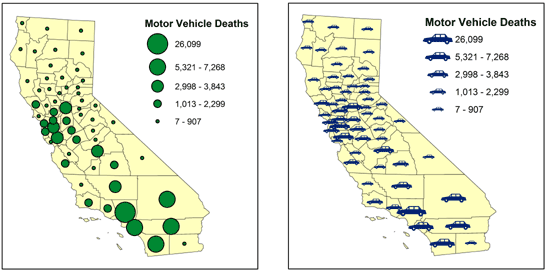
\includegraphics[height=5cm,keepaspectratio]{images/psm/symbols.png}
\caption[
    Two types of proportional symbol maps with different symbols \iacite{Dutton.2014}.
]{Two types of proportional symbol maps with different symbols.}
\label{fig:different-symbols}
\end{figure}

Another consideration in terms of symbol used is the fact, that squares and bars tend to run off the page with large values earlier than circles might \iacite{Dutton.2014}. \citeauthor{FLANNERY1971} introduced a scaling factor for proportional circles for better estimation of the value. However, this correction may not be very effective, because the correction itself does not consider the map context. A phenomenon related to the importance of context is known as the ebbinghaus illusion. Figure \ref{fig:ebbinghaus} on \pageref{fig:ebbinghaus} shows such an illusion. Both central circles actually have the same size, but because of the context of each side, the central circles appear different.

\begin{figure}[!htb]
\centering
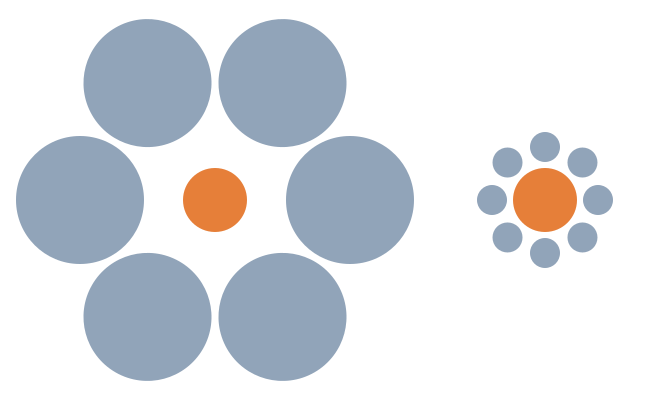
\includegraphics[height=5cm,keepaspectratio]{images/psm/ebbinghaus.png}
\caption[
    Ebbinghaus illusion, Urldate: 07.2016 \newline
    \small\texttt{\url{https://upload.wikimedia.org/wikipedia/commons/b/bc/Mond-vergleich.svg}}
]{Ebbinghaus illusion}
\label{fig:ebbinghaus}
\end{figure}

In order to combat the problem of value estimation, there are two major choices:
\begin{enumerate}
\item A legend could show proportional symbols which represent the different values of the mapped phenomenon. One possibility would be to display the smallest symbol, the largest symbol and some symbols at intermediate values.
\item Another alternative is to use range-graded symbols. Therefore the data needs to be classified, but in exchange the estimation problem is completly avoided. This alternative still needs consideration in the size of symbols, because each symbol should still be differentiable from each other.
\end{enumerate}

Based on the given knowledge about proportional and gradient symbol maps, it is possible to derive some main design principles:
\begin{itemize}
\item The estimation of the value of a symbol is key for this type of map. This is most easily accomplished with geometric symbols.
\item Use a legend with exmaples to increase the reader's ability to correctly estimate the value of a symbol.
\end{itemize}

A close related problem to the user's estimation problem is the actual scaling technique used. According to \citeauthor{Dent2008} the three most commong techniques used are
\begin{enumerate*}
\item absolute scaling,
\item apparent magnitude scaling and
\item range grading \iacite{Dent2008}.
\end{enumerate*}

\begin{enumerate}
\ditem{Absolute scaling} makes each symbol fit it's dat value on the scale being used. This means, that a symbol representing four items in a dataset is twice as big as a symbol representing two.
\ditem{Apparent magnitude scaling} compensates for human error interpretation in scale. Using this technique, a symbol having twice as much in value is not twice as big, because it would appear smaller, leading to interpretation error. This type of scaling takes this error into account and increased the size of a symbol by more than the proportional amount \iacite{Krygier.2007}.
\ditem{Range grading} classifies the data into a fixed amount of groups. Each group has a fixed range of values and the same symbol to represent. The groups only differ in the range of values they represent and the size of the symbols.
\end{enumerate}

The main advantage of a proportional symbol map is the flexibility it comes along with. Possible data can either be numerical or categorical nature. Even the way the data is used is adjustable. An item can be mapped on a precise location or to geographic areas, depending on the level of detail.
Comparing proportional symbol maps with dot density maps, one advantage is observable: the estimation problem of dot density maps is less tedious. However, if proportional symbol maps are put in comparison with choropleth maps, they also have an advantage: the size of the enumeration unit does not matter. This problem will be explained in detail in chapter \ref{s:choropleth} on page \pageref{s:choropleth}.

\sectionparagraph{Choropleth map}
Choropleth maps are extremely popular, probably the most common thematic map in use today. That's good because it means your audience is likely to understand them. One reason they're popular is that much of our geodata is reported by enumeration units, such as census data, and so we are accustomed to thinking of the world as divided into spatial units like census tracts, counties, and provinces. However, most cartographers would argue choropleth maps are over-used and commonly misused if the geographic phenomena being mapped aren't intrinsically tied to enumeration units: For example, communicable diseases, soil types, or age demographics don't care much about county lines or zip codes and rarely do they change abruptly at those human-created boundaries. By comparison, tax rates are very closely tied to enumeration units, do change abruptly, and make perfect sense as a choropleth map. The less the thing you are mapping is tied to enumeration units, the less sense a choropleth map makes.

These are maps, where areas are shaded according to a prearranged key, each shading or colour type representing a range of values. Population density information, expressed as 'per km²,' is appropriately represented using a choropleth map. Choropleth maps are also appropriate for indicating differences in land use, like the amount of recreational land or type of forest cover.



For continuous data, two mapping techniques are commonly used: choropleth and isarithmic mapping. This chapter will only cover choropleth mapping because the practical part of this thesis will not feature isarithmic mapping.


The choropleth method involves applying value or color
intensity to enumeration units (census tracts, counties, states, nations) based on some statistical
value. The higher an enumeration unit’s data value, the darker or more saturated the color value.
Fundamental to every choropleth method are the concepts of data standardization and
classification.
All choropleth data must be standardized. We repeat: a choropleth map may never – ever –
be used to map count data. If one maps raw data using the choropleth method, the visualization
will suffer from an inherent areal bias. Not all enumeration units are the same size; thus, some
enumeration units will naturally have more count data than others simply due to their areal
extent. For instance, Texas and California have greater populations than Rhode Island or
Connecticut. This should not be a surprise – Texas and California have huge areas compared to
the other two states. If you standardize the data by area, however, Connecticut and Rhode Island
are far more populated when it comes to the number of people per square kilometer. If you are
interested in comparing the raw number of people living in states, you should use proportional
symbols.
\label{s:choropleth}

\subsubsubsection{Multivariate Thematic Map Types}

\subsubsection{Map Scale}
\subsubsection{Map Projections}
\subsubsection{Map Generalization}
\subsubsection{Symbolization}
\subsubsection{Map Accuracy}
\label{s:map-accuracy}


\subsection{Geographic Visualization}
Chapter \ref{s:definitions-types} on page \pageref{s:definitions-types} already defines \ac{GeoVis}. It is closely related to \ac{InfoVis} and \ac{SciVis} and emphasises knowledge construction over knowledge storage or information transmission \iacite{maceachren:1997}. Owing to its roots in cartography, \ac{GeoVis} contributes to its related fields by way of the map metaphor, which "[\ldots] has been widely used to visualize non-geographic information in the domains of information visualization and domain knowledge visualization" \iacite{Jiang2005}.
In short, the thesis uses the term \ac{GeoVis} as a hypernym for the combination of exploratory data analysis, \ac{InfoVis}, \ac{SciVis}, thematic cartography and visual analytics.

\ac{GeoVis} are superior to traditional, static maps because they are not limited to exploration capabilities. They allow more interaction in maps, due to the ability of extending the basic layer of the map with user-experience abilities like zooming to change the visual appearance \iacite{Jiang2003}. These kinds of visualisations are also used in practical applications which are briefly outlined in this chapter.

\begin{description}

\item[Urban Planning] \hfill \\
Urbanists use \ac{GeoVis} to "[\ldots] model environmental interests and policy concerns of the general public" \iacite{Jiang2003}. \citeauthor{Jiang2003} also mention two examples, in which "[\ldots] 3D photorealistic representations are used to show urban redevelopment and dynamic computer simulations are used to show possible pollution diffusion over the next few years".
\citeauthor{Jiang2003} also describe that the widespread use of the internet by the general public impacts collaborative planning. The former way of planning in committee rooms or computer facility rooms can now be extended with a decentralised web platform. The use of the internet features two important aspects of planning:
\begin{enumerate*}
\item it already integrates various interactive and proactive techniques and
\item it is time and place independent.
\end{enumerate*}

\item[Environmental Studies] \hfill \\
\citeauthor{Danado2005} describe a system that is capable of simulating and visualising environmental processes collaboratively. In addition, the system has the ability to retrieve information while moving in real time. Thus each user can impact the simulation by adding or removing information to or from the model. The system also reacts on the changes the users made, therefore making it possible to explore a complex set of environmental data, affecting it with different actions and determine a best fit \iacite{Danado2005}.

\item[Forestry] \hfill \\
\citeauthor{Andrienko2007} present a system to visualise a large set of spatio-temporal data related to european forests. The innovative approach of this system is given by the interaction. Non-experts can change parameters in the system and explore the results. Furthermore \citeauthor{Andrienko2007} state their approach "[\ldots] uncovers a range of fundamental issues relevant to the broad field of \ac{GeoVis} and \ac{InfoVis} research \iacite{Andrienko2007}."

\citeauthor{Andrienko2007} also cited the two major problems as
\begin{enumerate}
\item the inability of the geovisualisers to convince the foresters of the efficiency of \ac{GeoVis} in their work and
\item the foresters' misgivings over the dataset's accessibility to non-experts engaging in "uncontrolled exploration".
\end{enumerate}

\item[Telecommunication] \hfill \\
\ac{GeoVis} are also very helpful in the area of telecommunication. Telegeography\footnote{https://www.telegeography.com/}, as an example for a company in that specific area, has an interactive submarine cable map. Figure \ref{fig:both-submarines} on page \pageref{fig:both-submarines} features an overview of this map (see figure \ref{fig:submarine}) and the interactivity (see figure \ref{fig:submarine-interactive}) which gives more information to the cable’s profile, including the cable’s name, ready-for-service date, length, owners, website, and landing points.

\begin{figure}[!htb]
  \captionsetup[subfigure]{justification=centering}
  \centering
  \begin{subfigure}[b]{0.4\textwidth}
    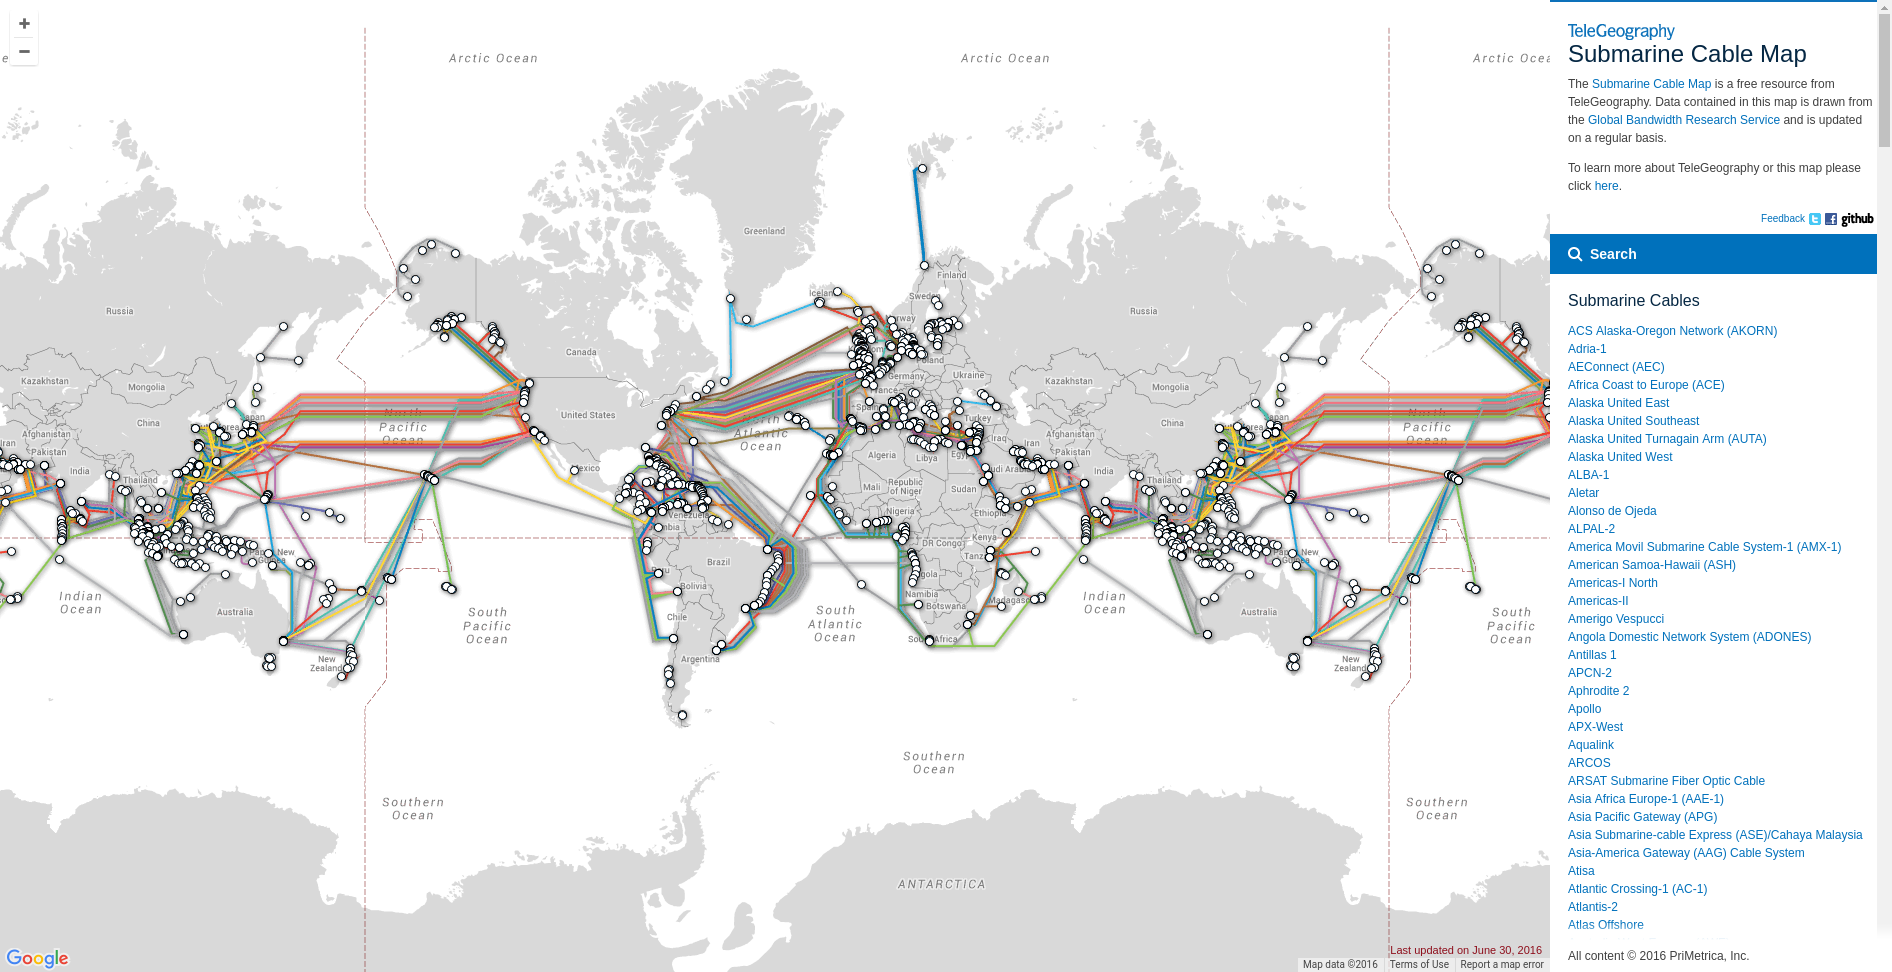
\includegraphics[width=\textwidth]{images/geovis/submarine.png}
    \caption[Overview of the submarine cable map]{Overview of the submarine cable map}
    \label{fig:submarine}
  \end{subfigure}
  \hfill
  \begin{subfigure}[b]{0.4\textwidth}
    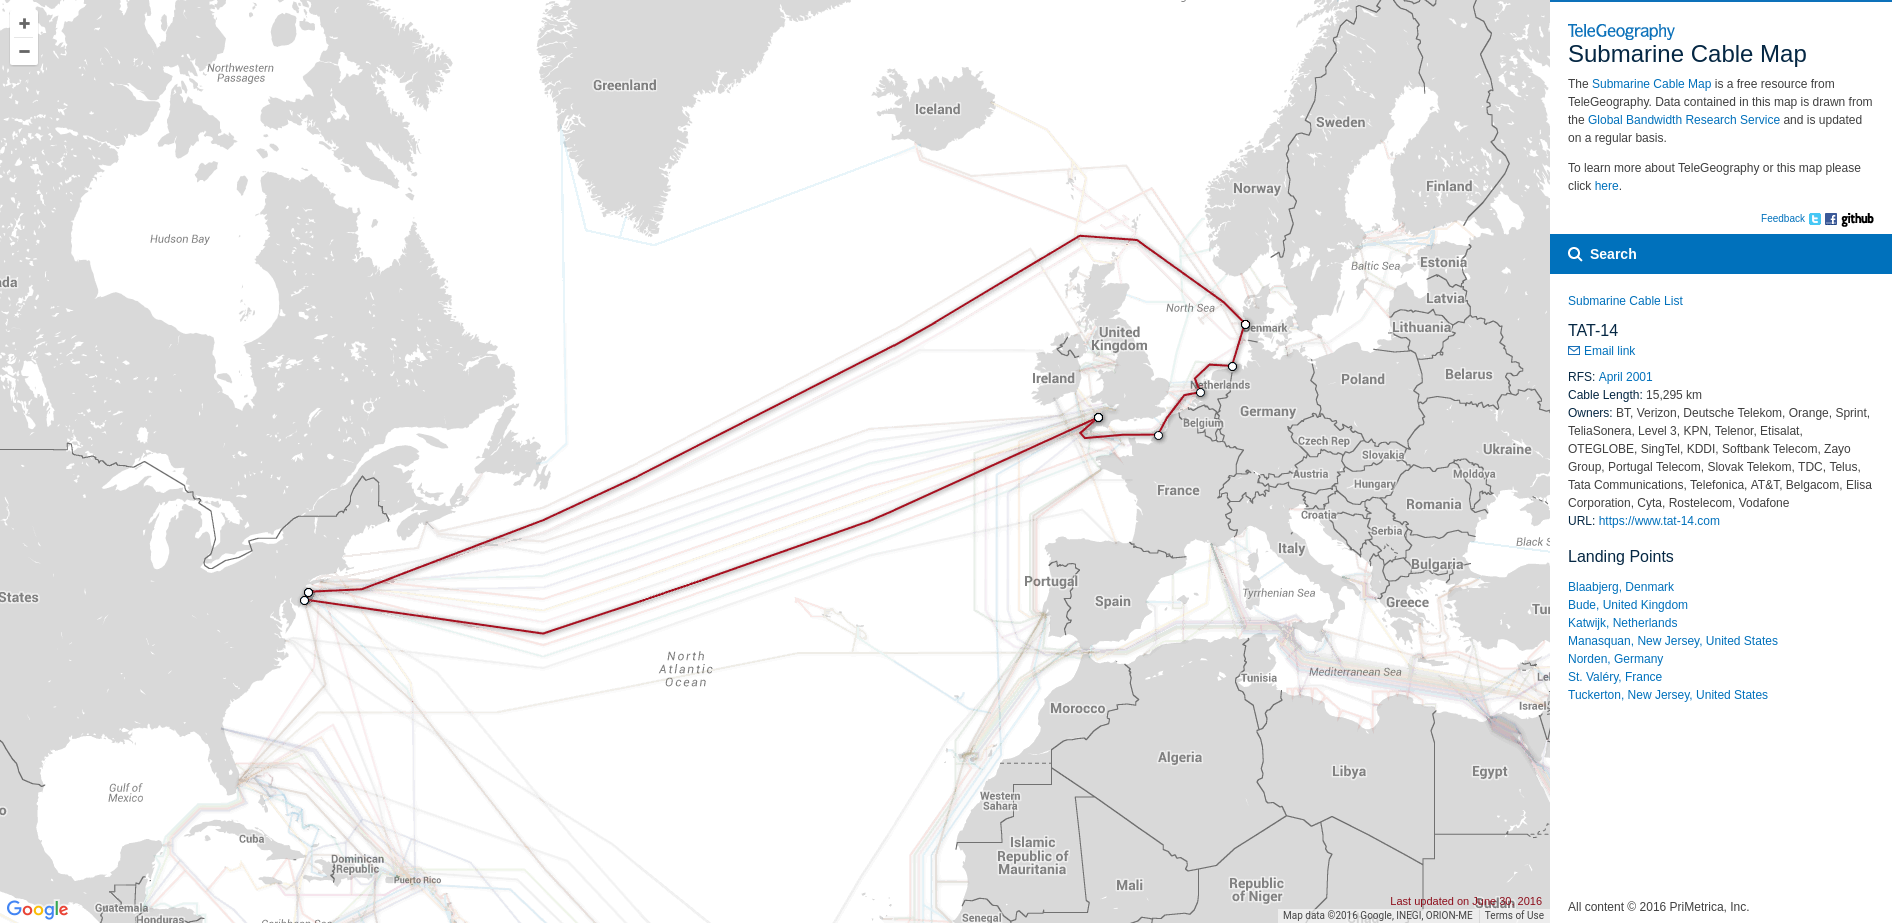
\includegraphics[width=\textwidth]{images/geovis/submarine-interactive.png}
    \caption[Interactivity of the submarine cable map]{Interactivity of the submarine cable map}
    \label{fig:submarine-interactive}
  \end{subfigure}
    \caption[
        TeleGeography’s free interactive submarine cable map, Urldate: 07.2016 \newline
    \small\texttt{\url{http://www.submarinecablemap.com/}}
    ]{TeleGeography’s free interactive submarine cable map}
  \label{fig:both-submarines}
\end{figure}

\item[E-commerce] \hfill \\
\ac{GeoVis} can be very useful in analysing data provided by e-commerce shops if they track orders-behaviour of their customers with some kind of geographical information. If such data is available and provided, it is possible to easily visualise the target group of a company on a map and therefore create knowledge and allow for generating hypothesis i.e. the next region for expansion.

\end{description}

\subsection{Interaction in visualizations}
\label{s:interaction}
When designing maps, there is one important distinction: designing maps for print versus the internet. For the first case, the design is for map readers, whereas for the latter case, it is for map users. The difference between readers and users lays in the interaction. This chapter focuses on a map designed for the internet and therefore allowing a lot more interaction. Users do not only interact but also manipulate web maps. Interaction for print maps would be moving a paper map closer or further away to one's eyes, or trim specific parts with scissors and so forth. The weakness of this kind of interaction is that the data on the map stays the same. However, zooming, selecting and moving a map on the internet actually allows for adapting the data shown \iacite{Muehlenhaus2014}.

As already mentioned in chapter \ref{s:definitions-types} on page \pageref{s:definitions-types}, \citeauthor{Shneiderman1996} published an often cited mantra \iacite{Shneiderman1996}:
\begin{quote}
"Overview first, zoom and filter, then details on demand."
\end{quote}

% MISSING BOOK: Information Visualization: Design for Interaction Spence 2007
% This mantra can also be used as a guideline for creating web maps with interaction.
% % Spence2007
% introduces a so called action cycle, which models an interactive exploration process of data. Small datasets, as well as complex and dynamic data can make use of this process in order to properly implement and integrate interaction.

% TODO - CHECK IF ENOUGH WORDS

The first part of this chapter will introduce some basic interaction methods and concepts. The second part will build upon the knowledge of the first part and maps the basic concepts to today's implementations with the focus on interaction with thematic maps.

\subsubsection{Overview First, Focus \& Context}
A natural way according to the mantra presented by \citeauthor{Shneiderman1996} to visualise a dataset is to start with an overview. This supports the user's understanding of the complexity and size of the whole dataset. However giving an overview first is also dependant on the dataset. Imagine a \ac{GIS} like OpenStreetMap\footnote{See \href{https://www.openstreetmap.org}{https://www.openstreetmap.org}} would show random location, e.g. a valley with a lot of detail as a starting point. There are two contrary use cases where such a starting point would make sense or not.
\begin{enumerate}
\item If the dataset the map is based on only contains data of that specific ``random'' valley shown, it definitely makes sense to only show that valley. The dataset does not contain information about all valleys, therefore making it unnecessary to show the whole map of the earth as an overview first.
\item The use case mentioned already, implicitly explains a bad use case of a random starting point. If a dataset inheres structure, like a whole map of the world, it is not useful to start at a specific location, therefore showing an overview of the earth first makes more sense.
\end{enumerate}

Focus and context describes a concept that puts a specific part of dataset, called subset, in focus while still showing an overview of the other part. One example implementation of this concept are fisheye views, originally developed by \citeauthor{Furnas:1986} \iacite{Furnas:1986}. Figure \ref{fig:focus} on page \pageref{fig:focus} shows a modern implementation of the focus and context concept based on a fisheye view. The focus in this Figure is set somewhere between the blue and orange circle in the middle of the Figure. This part is magnified as one can see on the circle size, while the ones further away are smaller and a little distorted.

\begin{figure}[!htb]
\centering
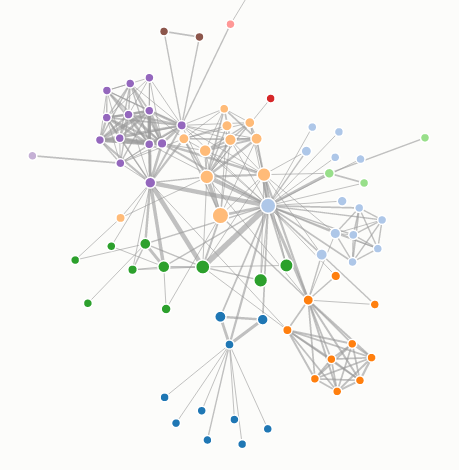
\includegraphics[height=5cm,keepaspectratio]{images/methods/interaction/focus.png}
\caption[
    The focus and context concept based implemented with a fisheye view, Urldate: 07.2016 \newline
    \small\texttt{\url{https://bost.ocks.org/mike/fisheye/}}.
]{The focus and context concept implemented with a fisheye view. The blue node in the center of the Figure and the yellow node left to it are bigger compared to the other ones. This is due to the magnification of this part.}
\label{fig:focus}
\end{figure}

\citeauthor{Kosara2003} categorise the aforementioned method as distortion-oriented \iacite{Kosara2003}. Other techniques they list are summarised below:
\newpage
\begin{description}
\item[Overview methods] show the context in a separate layer in the same place \iacite{Kosara2003}.
\item[Filtering] shows additional information of particular subparts e.g. with a magic lens. They provide an object of any shape that can move freely. The area it covers is shown with more information \iacite{Bier:1993}.
\item[In-Place techniques] are similar to filtering without the requirement of a lens. The implementation of the technique points out information to the user, e.g. by highlighting. The program can also take the initiative and point the user to interesting data \iacite{Kosara2003}.
\end{description}


\subsubsection{Details on Demand}
Showing detailed information upon interaction on a dot map based on a dataset with 10000 data items describes the concept of showing details on demand. It would be infeasible to show details on all entries, as the screen-space is limited. Even with unlimited screen-space it, would drastically worsen the readability of the map. \citeauthor{Ahlberg:1996} explains one possible way of implementing this concept. His approach is to only show objects that match certain criteria and are therefore likely of interest to the user. However, the user needs to start this task first with some kind of interaction, e.g. clicking on a visual object of a specific type. The additional information is then shown in a pop-up window \iacite{Ahlberg:1996}.



\subsubsection{Multiple Views, Linking \& Brushing}
\label{s:linking-brushing}
Multiple view systems are defined by using several views on the same dataset, but with different aspects of it for each visualization. Practical applications of all kinds make use of such a system, e.g. \ac{CAD} and \ac{GIS}. Even though the possibility of using multiple views on the same dataset is trivial, the implementation and necessary amount of interaction is not \iacite{Kosara2003}.

\citeauthor{Baldonado2000} present four design rules wheter or not multiple view systems are appropriate for the specific task \iacite{Baldonado2000}:

\begin{enumerate}

\ditem{Diversity} \hfill \\
If the given dataset consists of attributes with different types, multiple levels of abstraction, and so forth, a multiple view system can be created. A single view would be overloaded with the given dataset because of the significant cognitive overhead created. The user would need to simultaneously comprehend and assimilate a multitude of diverse data.

\ditem{Complementarity} \hfill \\
Multiple view systems support visual comparability. They should be used if showing correlations and/or disparities is important, because they leverage multiple perceptual capabilities to improve understanding of relations among views.

\ditem{Decomposition} \hfill \\
Showing different attributes at the same time provides insight in different dimensions. This rule is related to the "divide and conquer" principle: the amount of data a user needs to consider at one time is reduced, thus aiding memory.

\ditem{Parsimony} \hfill \\
Multiple views build upon the cost of switching context and increasing complexity. The learning cost of a user, aswell as computational and display space costs of several views must be justifiable.

\end{enumerate}

Multiple view systems are often used for focus and zoom, e.g. for showing the focus and contex in seperate windows. \citeauthor{Robert:1998} describe a system based on this concept \iacite{Robert:1998}.

\citeauthor{Martin:1995} describe brushing as the process of selecting specific data items or groups of items to highlight them \iacite{Martin:1995}. Usually this process is initiated by directly interacting with the view using the mouse. Two possible manual interactions are opening a rectangular region of interest or clicking on a specific data items. It can also be accomplished without interacting with the visualization itself by using sliders, select-boxes or even complex means like selecting a cluster \iacite{Kosara2003}.

However, using the brushing technique is not sufficient when exploring complex data efficiently. Linking describes the concept of exchanging information about which points are brushed. This concept is essential when using brushing and multiple view systems together. With this combination, a user can easily see the same points brushed in different views on the data \iacite{Kosara2003}.



\subsubsection{Animations and Transitions}
In order to understand transition referring to visualizations, it is important to point out the difference between transition and animation. Even though these two terms are often substituting each other, they follow two different concepts \iacite{Muehlenhaus2014}:

According to the Merriam Webster Online Dictionary\footnote{See \href{http://www.merriam-webster.com/}{Merriam Webster Dictionary}} an animation is a way of making a movie by using a series of drawings, computer graphics or photographs that are slightly different from one another and that when viewed quickly one after another create the appearance of movement. Transition, however, is a movement, development, or evolution from one form, stage, or style to another.

With these definitions, it is easy to distinguish the two terms. Animation is the process of making any kind of movement visible to a user, whereas transitions in visualizations make use of animations to show e.g. the change of visual appearance.

\citeauthor{Thrower1959} was the first one to combine the research fields of cartography with animation. He describes the process of bringing e.g. population growth with animation on a map \iacite{Thrower1959}. However, animated cartography remained a bit of an oddity that was experimented with. This fact could not be changed even with the rise of the household \ac{PC}. Nonetheless, the mass adoption of the internet could counteract the rare usage of map animation \iacite{Muehlenhaus2014}.

This chapter furthermore describes considerations when designing animated maps. Animation can basicly be broken down into two broad types:

\begin{enumerate}
\ditem{Stop-Frame Animation} \hfill \\
This type of animation is also known as stop motion. Every frame of this type of animation is designed separately. After many pictures and movements are made, all pictures are in the order they were taken. The rate of change for each picture heavily influences the cognition of the animation \iacite{Faroudja1991}.
\ditem{Tweening} \hfill \\
    This term bears its name from the word "betweening". It describes the process of interpolating movement between key frames, thus creating smoother animations compared to the stop-frame method \iacite{Muehlenhaus2014}.
\end{enumerate}

\citeauthor{DiBiase1992} identified three new visual variables dealing specifically with animation \iacite{DiBiase1992}:

\begin{enumerate}

\ditem{Duration} defines the temporal length of how long a particular frame in an animation is shown. Imagine a dataset containing decennial census of population data and an animation set to 24 frames per second. To give each map user the ability to conceive each decade, it is needed to show it at least for some seconds. For the sake of convenience a duration of 2 seconds is assumed to be enough. Therefore, it is needed to show each decennial census data for 48 frames, resulting in a 2 second duration \iacite{Muehlenhaus2014}.

\ditem{Rate of Change} represents how quickly an image is morphed into the next attribute. In general, it denotes the magnitude of an attribute divided by the duration. This basically means, that it is needed to know how much the animated image being represented changes from frame to frame \iacite{Muehlenhaus2014}.

\ditem{Order}
Rather than animating data in the order they are given, they can be reorganized first by a specific attribute. For example, one could show all countries with a high population first, before showing small ones \iacite{Muehlenhaus2014}.

\end{enumerate}

\citeauthor{Muehlenhaus2014} also mentions differnt types of map animations. He says weather forecasts are the most common use case for map animations. Thus deriving the term temporal animation for this kind of animation seems appropriate. Albeit showing change over time seems trivial, people do not always interpret the resulting animation accurately. He suggests the use of temporal animations for showing broad patterns of change in a dataset. However, the animation should either show broad changes in a small scale or detailed changes in a large scale. This heavily impacts the user's perception and interpretation of the animation, including "change blindness". This means, that obvious changes in a map are missed due to focusing something else in the map. In order to combat the problem of change blindness, he \citeauthor{Muehlenhaus2014} names three different design principles \iacite{Muehlenhaus2014}:

\begin{enumerate}

\item \textbf{Animation duration} should be kept short in order to not overwhelm a user's short-term memory. Temporal animations should not take longer than 30 seconds to a minute, especially when showing changes in data, which are not narrative in nature. If this principle is ignored, data retention will be nullified \iacite{Muehlenhaus2014}.

\item \textbf{Data simplification} denotes the amount of animated attributes used. Showing more than four attributes in an animation results in visual overstimulation \iacite{Ware2008}.

\item \textbf{Control} needs to be given to the user. This can be achieved in many ways, e.g. by providing a pause or play button for an animation \iacite{Muehlenhaus2014}.

\end{enumerate}

Another type of animation \citeauthor{Muehlenhaus2014} mentions is the so called zoom animation. This type basically follows the main visual information seeking mantra of \citeauthor{Shneiderman1996}. If the purpose of an animation is to show a specific part of the data, it should start off by giving an overview. The animation is either started programmatically or manually and animates the focus to a specific part of the data. Control can ge given to the user in form of freely moving around in the map or providing zoom buttons.

However, the mentioned types of animations are only based on a single visualization. This thesis will use animation in a transition of one type of map visualization to another. First, this should help to understand how the map is created. Second, some map visualizations are based on aggregations and therefore, the animation should show if this aggregation is understandable and interpretable.



\subsection{State-of-the-art application analysis}